Last time, we wrote down the equation relating the scale factor $a$ to the content of spacetime:
$$\dot \rho = -3(p+\rho)\dot a/a.$$

Some examples of the stuff in spacetime include dust ($p=0,\rho_M=\rho_0 a_0^3/a^3$), radiation ($p=\rho/3$, with $\rho_{rad}=\rho_0 a_0^4/a^4$, and dark energy ($p=-\rho$, $\rho_\Lambda=$constant).
But what we observe is that in an expanding universe, radiation is thus diluted faster ($a^{-4}$) than matter ($a^{-3}$), which is diluted faster than dark energy.

Now recall that we have written the Einstein equations
$$R_{ab}-\frac{1}{2}R g_{ab}+\Lambda g_{ba}=8\pi T_{ab},$$
where we have supposed the metric separates into a time component and a scaled spatial component,
$$ds^2=-dt^2+a^2(t) d\sigma^2.$$
Now using the form of $T_{ab}$ in terms of $\rho,p$, we get
$$4\pi(\rho+3p)-\Lambda=-3\ddot a/a,$$
which can be written as
$$3\dot a^2=8\pi \rho a^2 +\Lambda a^2 -3k.$$
This is sometimes known as the Raychaudhuri equation or the energy equation.%where does this come from? Check Sean Carroll later

In the absence of matter, there is just $\Lambda$ to govern the curvature and expansion. $\Lambda >0$ gives de Sitter space, $\Lambda=0$ Minkowski space, and $\Lambda <0$ anti de Sitter space. What happens if we put some matter in?

If we now take dust with $p=0$ and start with a $\Lambda=0,k=0$ universe, we get
$$a(t)\sim t^{2/3},$$
a power law. Suppose we take boundary conditions $a(t_0)=a_0.$ Then
$$a(t)=a_0 (t/t_0)^{2/3},$$
and we can relate the density to time,
$$\rho_0=\frac{1}{6\pi t_0^2}.$$
That is, we can relate $\rho_0$ the density at $t_0$ to the age of the universe. But notice that as we rewind to $t=0$, the curvature (or equivalently the density) blows up-- spacetime becomes singular. This turns out to be fairly generic behavior in the absence of a cosmological constant. Theorems of Hawking and Penrose in fact guarantee that in an expanding universe with ordinary matter ($\Lambda=0$), there must be an initial singularity. %maybe add a link here later
Like most singularities, there is really nothing more we can say about it.

Let's now consider the $k=1$ case, still for dust ($\Lambda=0,p=0$). The Raychaudhuri equation now gives us
$$\dot a=\sqrt{\frac{8\pi \rho_0 a_0^3}{3a}-k}.$$ If we now make the substitution $a=\frac{8\pi \rho_0 a_0^3}{3}\sin^2\theta$, the equation becomes
$$\frac{16\pi \rho_0 a_0^3}{3} \int \sin^2\theta d\theta =t,$$
which has the solution
$$\frac{8\pi \rho_0 a_0^3}{3}(\theta-\frac{1}{2}\sin 2\theta)=t.$$ Thus
$$a(t)=\frac{8\pi \rho_0 a_0^3}{3}\sin^2\theta,$$
which is the formula for a cycloid. The universe therefore expands out to some maximum scale at $\theta=\pi/2$, and then contracts back to a singularity at $t=\pi$.

What if $k=-1$? Then we ought to modify the sine to a sinh, $$a=\frac{8\pi\rho_0 a_0^3}{3}\sinh^2 \theta.$$
The solution is now
$$t=\frac{9\pi\rho_0 a_0^3}{3}(\frac{1}{2}\sinh 2\theta -\theta),$$
which leads to continuous expansion. It is at first independent of $k$: for small $t$,
$$a(t)\sim t^{2/3}.$$
But at late times, $k=-1$ looks like linear expansion.

What we find is that it is hard to measure $k$ when $t$ is small-- at early times, all expansions look pretty similar in their scaling-- see Fig. \ref{fig:flrw_metric}.

\begin{figure}
    \centering
    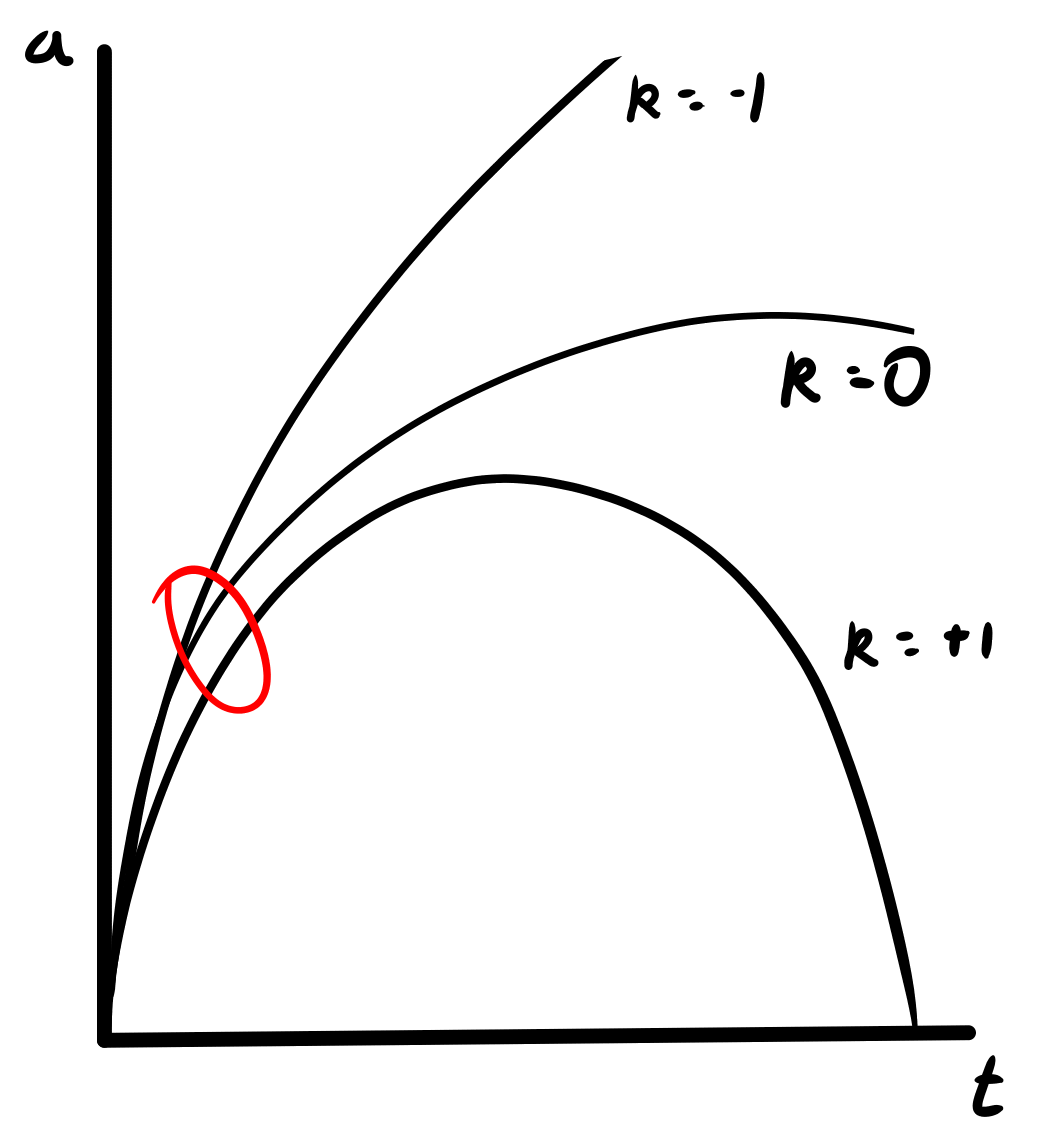
\includegraphics{2018/11/20181114_scalefactor.png}
    \caption{The scale factor as a function of time. We have written the metric as $ds^2=-dt^2 +a^2(t) d\sigma_k^2$, where $d\sigma_k^2$ is a purely spatial metric. The spatial part can be positively curved ($k=+1$), negatively curved ($k=-1$), or flat ($k=0$). At early times (the circled red region), all three scenarios expand similarly, but the $k=+1$ solution eventually contracts back to a singularity, while the $k=0$ and $k=-1$ solutions expand forever. Experimentally, we cannot yet distinguish between which of these scenarios describes our universe.}
    \label{fig:flrw_metric}
\end{figure}

\subsection*{Gravitational radiation} Just as Maxwell's equations in vacuum have plane wave solutions, we expect that Einstein's equations in vacuum might also reasonably have some wave solutions. We can treat these solutions using perturbation theory. Think about small perturbations to the metric,
$$g_{ab}=g_{ab}^{(0)}+h_{ab},$$
and let's work in linear order in $h$.

Then we can expand the Einstein equations accordingly. For instance,
$$\delta R_{ab}=-\frac{1}{2}\Box h_{ab}+\frac{1}{2}\nabla_d \nabla_a h^d_b +\frac{1}{2}\nabla_d \nabla_b h^d_a -\frac{1}{2}\nabla_a \nabla_b h,$$
with $h=h_{ab}{g^{(0)}}^{ab}$. Note that the covariant derivatives $\nabla$ are taken with respect to the original unperturbed metric $g^{(0)}$. The variation of the Einstein equations is therefore
$$\delta R_{ab}-\frac{1}{2}\delta R g_{ab}^{(0)} -\frac{1}{2}R h_{ab}=8\pi T_{ab}.$$
 Here, we think of $T_{ab}$ as the source of gravitational radiation, so $T_{ab}$ is of order $h$.

To simplify somewhat, we take $g^{(0)}$ to be Minkowski space and work in $t,x,y,z$ coordinates. Thus $\nabla_a$ becomes a partial derivative and $\Box$ is just the flat space wave operator. Our equations simplify to
$$-\Box h_{ab}+\p_d \p_a h^d_b +\p_d \p_b h^b_a -\p_a \p_b h=16\pi T_{ab},$$
which is the analog of Maxwell's equation-- written in terms of a vector potential, that looks like
$$\Box A^a -\p_b \p^a A^b=-\mu_0 j^a.$$
It is often convenient to solve Maxwell's equations with an appropriate choice of gauge. Let us try to find something equivalent for our Einstein equations.

Suppose one makes a coordinate transformation
$$x^a \mapsto {x'}^a = x^a +\epsilon^a.$$
We previously found that if the line element is invariant, this changes the metric by $\nabla_a \epsilon_b +\nabla_b \epsilon_a$. When such transformations were isometries (leave the metric unchanged), these $\epsilon$s just solved Killing's equation. In our problem, this changes the metric by
$$\p_a \epsilon_b +\p_b \epsilon_a.$$

Thus $h'_{ab}=h_{ab}+\p_a \epsilon_b +\p_b \epsilon_a$ represents the same physical perturbation, and we shall choose $h'_{ab}$ to obey
$$\p_a({h'}^{ab}-\frac{1}{2}\eta^{ab}h')=0,$$
which we call the \term{harmonic gauge}. This is analogous to setting $\p_a A^a =0$ in electrodynamics.

Can we always do this? If we expand out this expression, we find that
$$0=\p_a({h'}^{ab}-\frac{1}{2}\eta^{ab}h')=\p_a(h^{ab}-\frac{1}{2}\eta^{ab}h)+\p_a \p^a \epsilon^b +\p_a \p^b \epsilon^a -\frac{1}{2} \eta^{ab} \p_a \underbrace{(2\p_c \epsilon^c)}_{h'}.$$
These last two terms cancel, so setting this gauge is equivalent to solving
$$\Box \epsilon^b = -C^b$$ for
$C^b=\p_a(h^{ab}-\frac{1}{2}\eta^{ab}h).$
But we can always solve this equation by constructing a Green's function for $\Box$, so one can always choose this gauge. We'll show this explicitly in the next lecture.

\subsection*{The Green's function for $\Box$} Generically, our equation takes the form
$$-\frac{\p^2 \epsilon^b}{\p t^2}+\nabla^2 \epsilon^b =-C^b.$$
Here, $\epsilon^b, C^b$ are functions of $\vec x,t$. Let us take the Fourier transform and write in $\vec p,\omega$ variables as
$$\hat \epsilon(\vec p,\omega)=\int d^3x dt \epsilon(\vec x,t) e^{-i\omega t +i\vec p \cdot x}.$$
Time derivatives bring down $\omega$s and $\nabla$s bring down $\vec p$,s so our equation in Fourier space reduces to
$$(\omega^2-\vec p^2) \hat \epsilon(\vec p, \omega)=-\hat C(\vec p, \omega).$$
Thus we rewrite
$$\hat \epsilon(\vec p, \omega)=-\frac{\hat C(\vec p,\omega)}{\omega^2-\vec p^2}.$$
We need only take the inverse Fourier transform to get us back to real space.